\documentclass[tikz, border=10pt]{standalone}
\usepackage{tikz}
\usetikzlibrary{shapes.geometric, arrows.meta, positioning, fit, backgrounds}

\definecolor{grucolor}{RGB}{52, 120, 190}
\definecolor{normcolor}{RGB}{120, 90, 170}
\definecolor{addcolor}{RGB}{80, 80, 80}
\definecolor{arrowcolor}{RGB}{60, 60, 60}
\definecolor{bgblock}{RGB}{245, 248, 255}

\tikzset{
  block/.style={rectangle, rounded corners=4pt, minimum width=3.2cm, minimum height=0.75cm, text centered, font=\small\bfseries, draw, thick},
  normblock/.style={block, fill=normcolor!20, draw=normcolor!70, text=normcolor!80!black},
  grublock/.style={block, fill=grucolor!20, draw=grucolor!70, text=grucolor!80!black},
  addblock/.style={circle, minimum size=0.55cm, text centered, font=\small\bfseries, fill=addcolor!15, draw=addcolor!60, text=addcolor},
  ioblock/.style={rectangle, rounded corners=2pt, minimum width=3.2cm, minimum height=0.6cm, text centered, font=\small, fill=gray!15, draw=gray!50},
  arr/.style={-{Stealth[length=5pt]}, thick, color=arrowcolor},
  skiparr/.style={-{Stealth[length=5pt]}, thick, color=addcolor!70, dashed}
}

\begin{document}
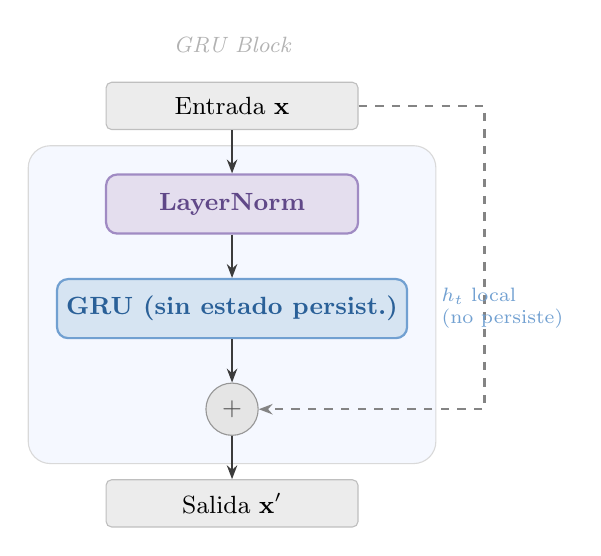
\begin{tikzpicture}[node distance=0.55cm]

  \node[font=\footnotesize\itshape, text=gray!60] (title) {GRU Block};
  \node[ioblock, below=0.25cm of title] (input) {Entrada $\mathbf{x}$};

  \node[normblock, below=of input]      (ln1)  {LayerNorm};
  \node[grublock,  below=of ln1]        (gru)  {GRU (sin estado persist.)};
  \node[addblock,  below=of gru]        (add1) {$+$};

  \node[ioblock, below=of add1]         (output) {Salida $\mathbf{x}'$};

  \draw[arr] (input)  -- (ln1);
  \draw[arr] (ln1)    -- (gru);
  \draw[arr] (gru)    -- (add1);
  \draw[arr] (add1)   -- (output);

  \draw[skiparr] (input.east) -- ++(1.6,0) |- (add1.east);

  \node[font=\scriptsize, text=grucolor!70, right=0.3cm of gru, align=left]
    {$h_t$ local\\(no persiste)};

  \begin{scope}[on background layer]
    \node[fill=bgblock, draw=gray!30, rounded corners=8pt, inner sep=10pt,
          fit=(ln1)(gru)(add1)] (border) {};
  \end{scope}

\end{tikzpicture}
\end{document}
